\chapter{Systemdesign}

\section{Architekturüberblick}
Gesamtsicht auf die Architektur der Lösung (Backend, Frontend, Datenbank).

\begin{figure}[!h]
    \centering
    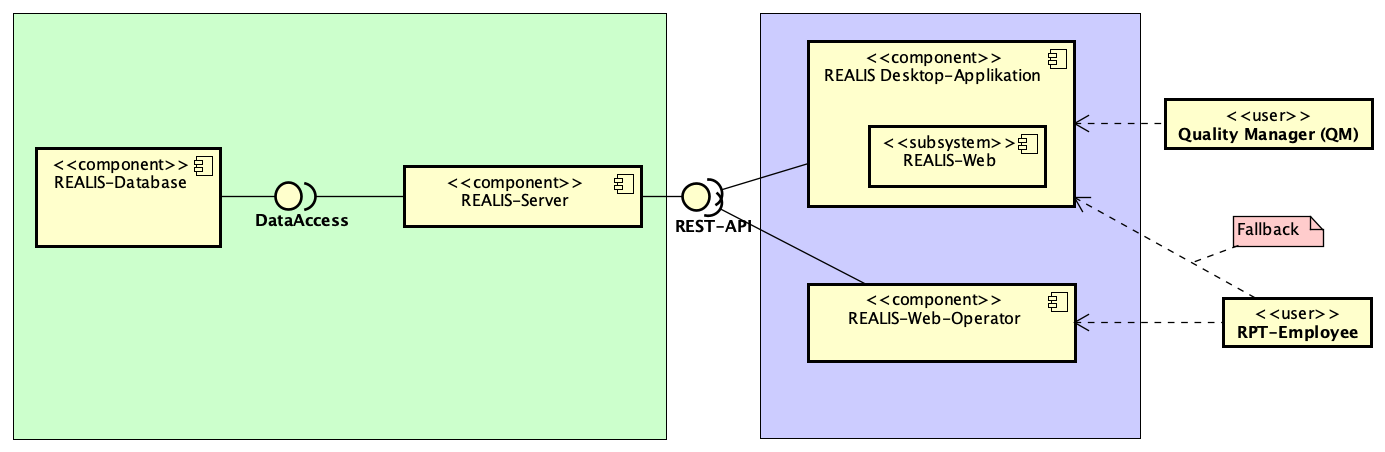
\includegraphics[width=1\textwidth]{bilder/REALIS-Komponentendiagramm.png}
    \caption{REALIS Komponentendiagramm}
    \label{fig:realis-komponentendiagramm}
\end{figure}

Da der Feasibility Check als Funktionalität in die bestehende Software-Applikation \gls{REALIS} integriert werden soll, ist es notwendig, die bereits verwendeten Technologien und Programmiersprachen zu übernehmen, um eine nahtlose Integration zu gewährleisten.

Eine Evaluierung alternativer Technologien, die möglicherweise besser für die Applikation geeignet wären, wurde daher nicht durchgeführt. Stattdessen orientiert sich die Umsetzung strikt am bestehenden System.

Für das Datenbankdesign kommt eine Oracle-Datenbank mit SQL zum Einsatz. Die Backend-Logik wird in der objektorientierten Programmiersprache C\# implementiert. Für das Frontend wird das Webapplikationsframework Angular verwendet, das auf TypeScript basiert. Angular ermöglicht eine parallele Entwicklung sowohl für Webanwendungen als auch für native Mobilapplikationen.

\section{Datenbankdesign}
Struktur der Oracle-Datenbank, wichtige Tabellen und Beziehungen.

\begin{figure}[!h]
    \centering
    \makebox[\textwidth]{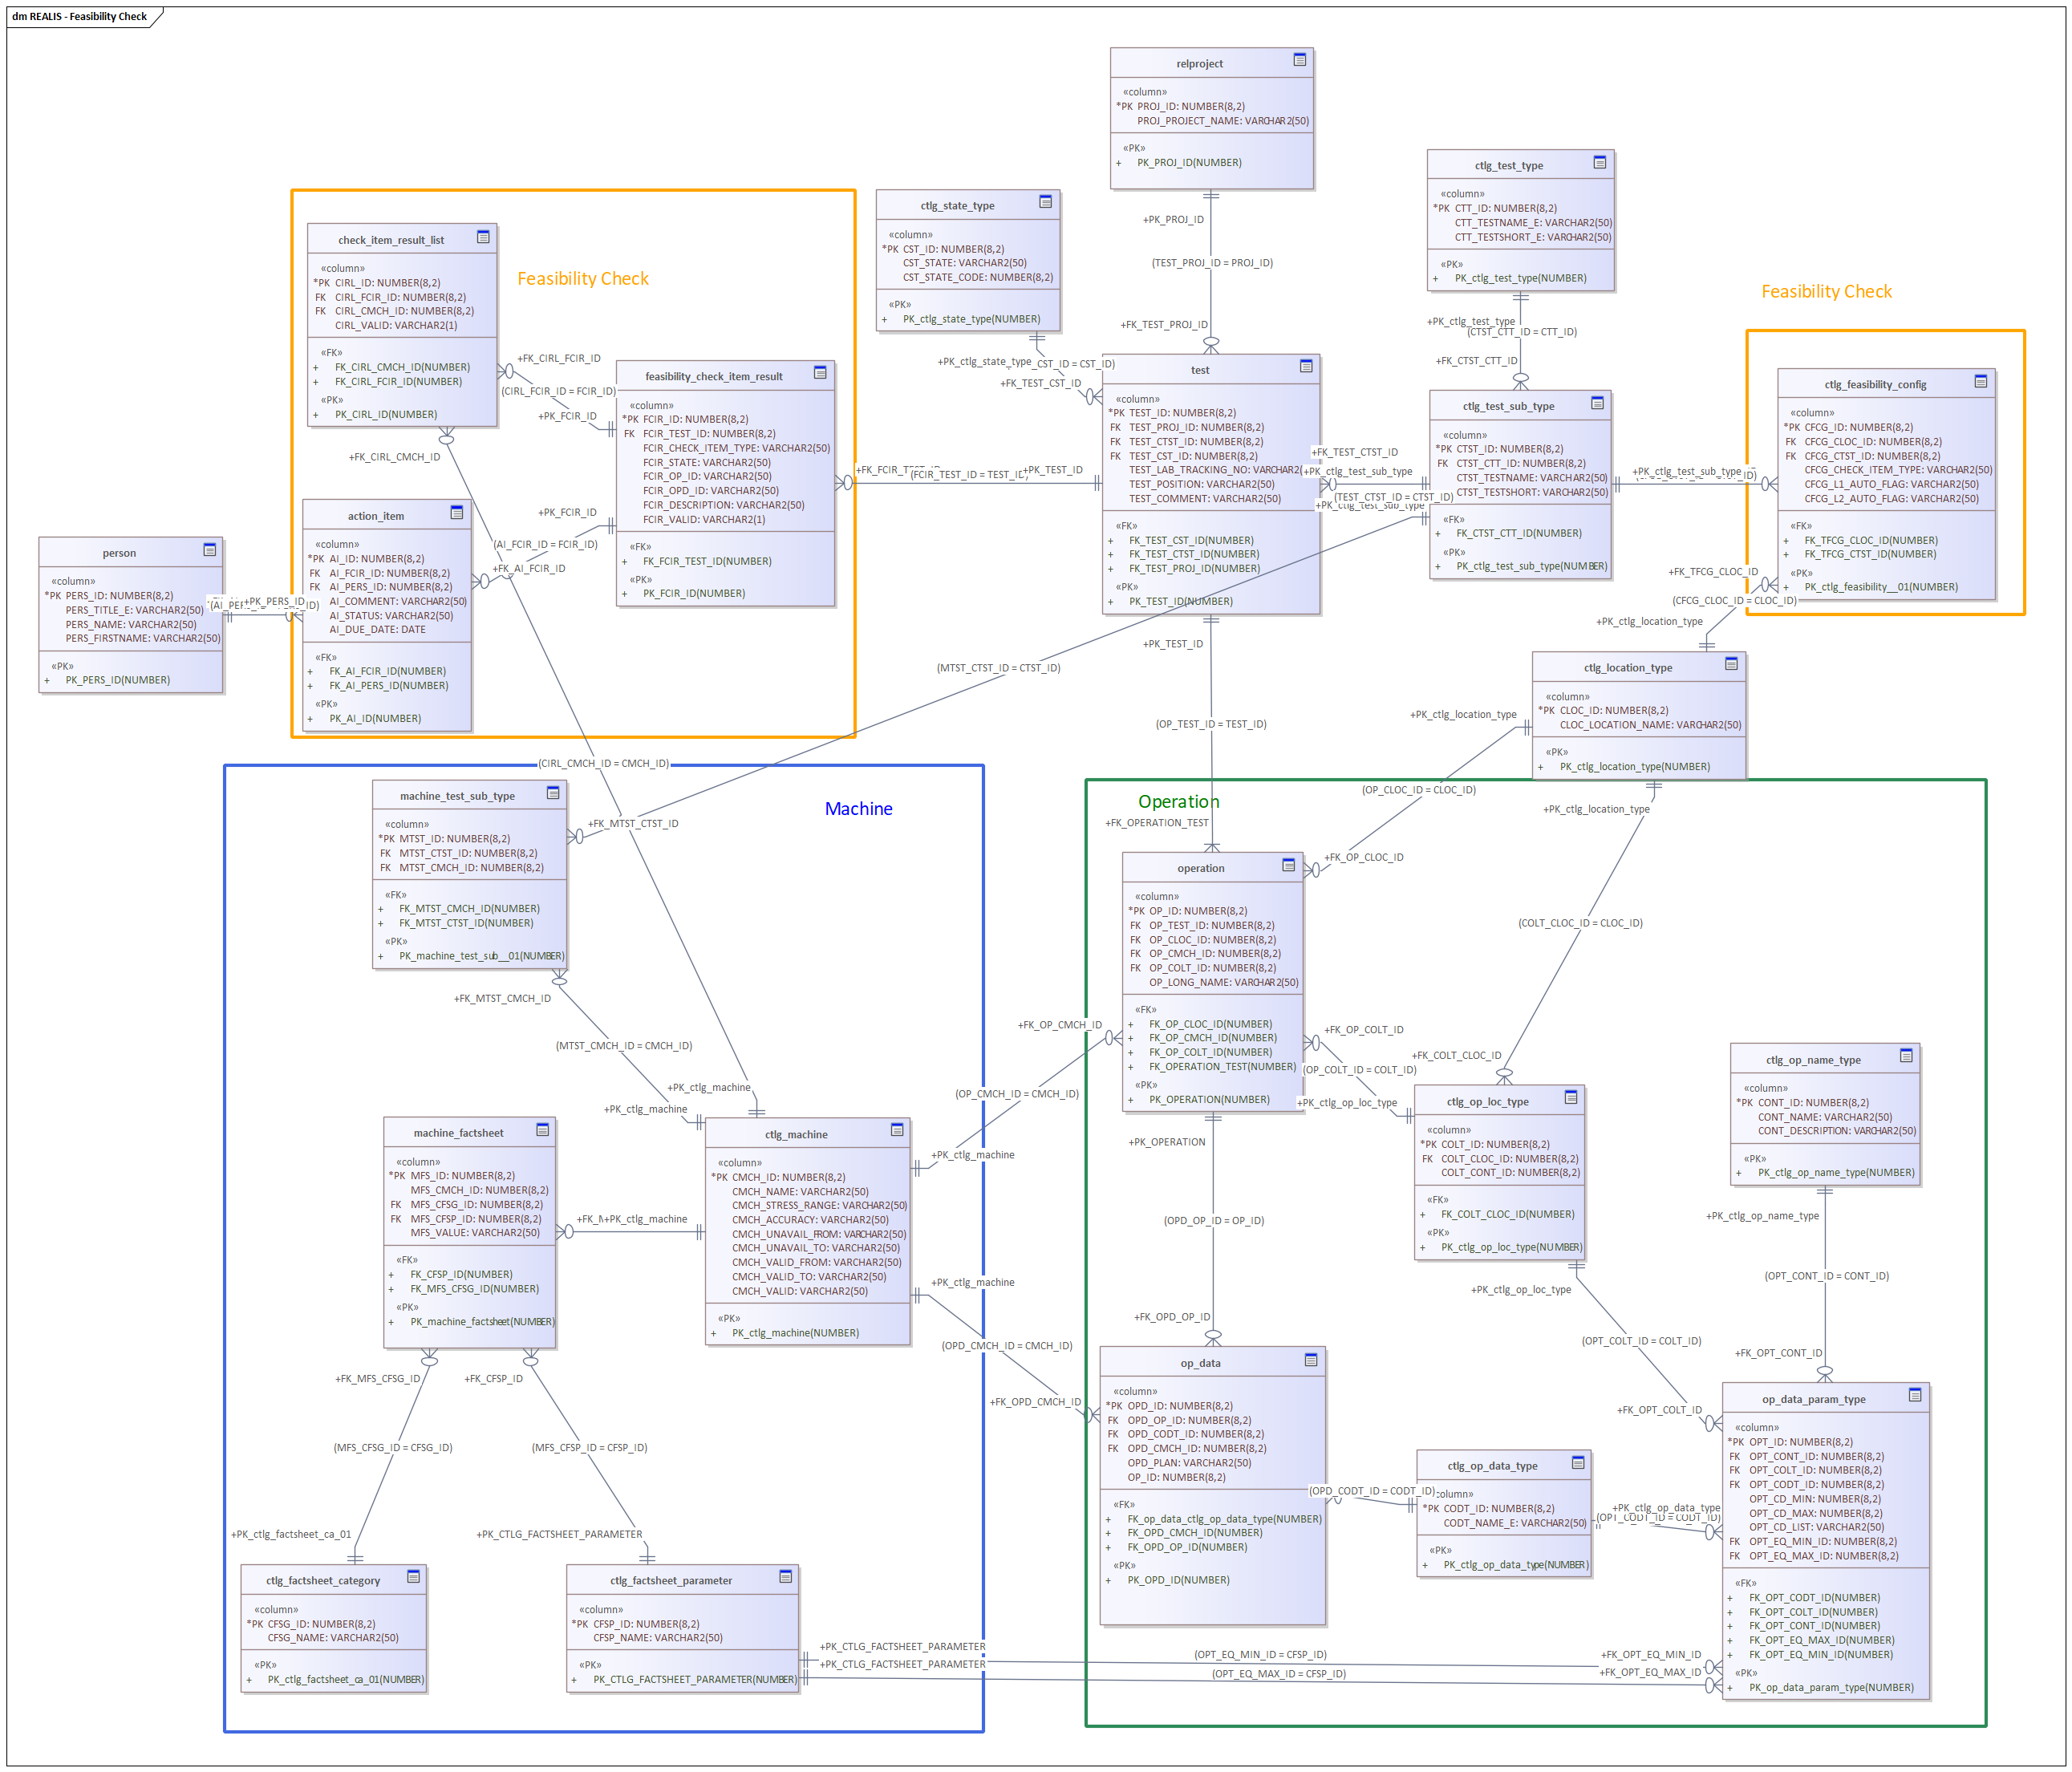
\includegraphics[width=0.98\paperwidth]{bilder/REALIS-Datenbankmodell.png}}
    \caption{REALIS Datenbankdesign}
    \label{fig:realis-datenbankdesign}
\end{figure}
\section{Backend-Logik}
Beschreibung der C\#-Implementierung, inklusive wichtiger Klassen und Methoden.

\begin{figure}[!h]
    \centering
    \makebox[\textwidth]{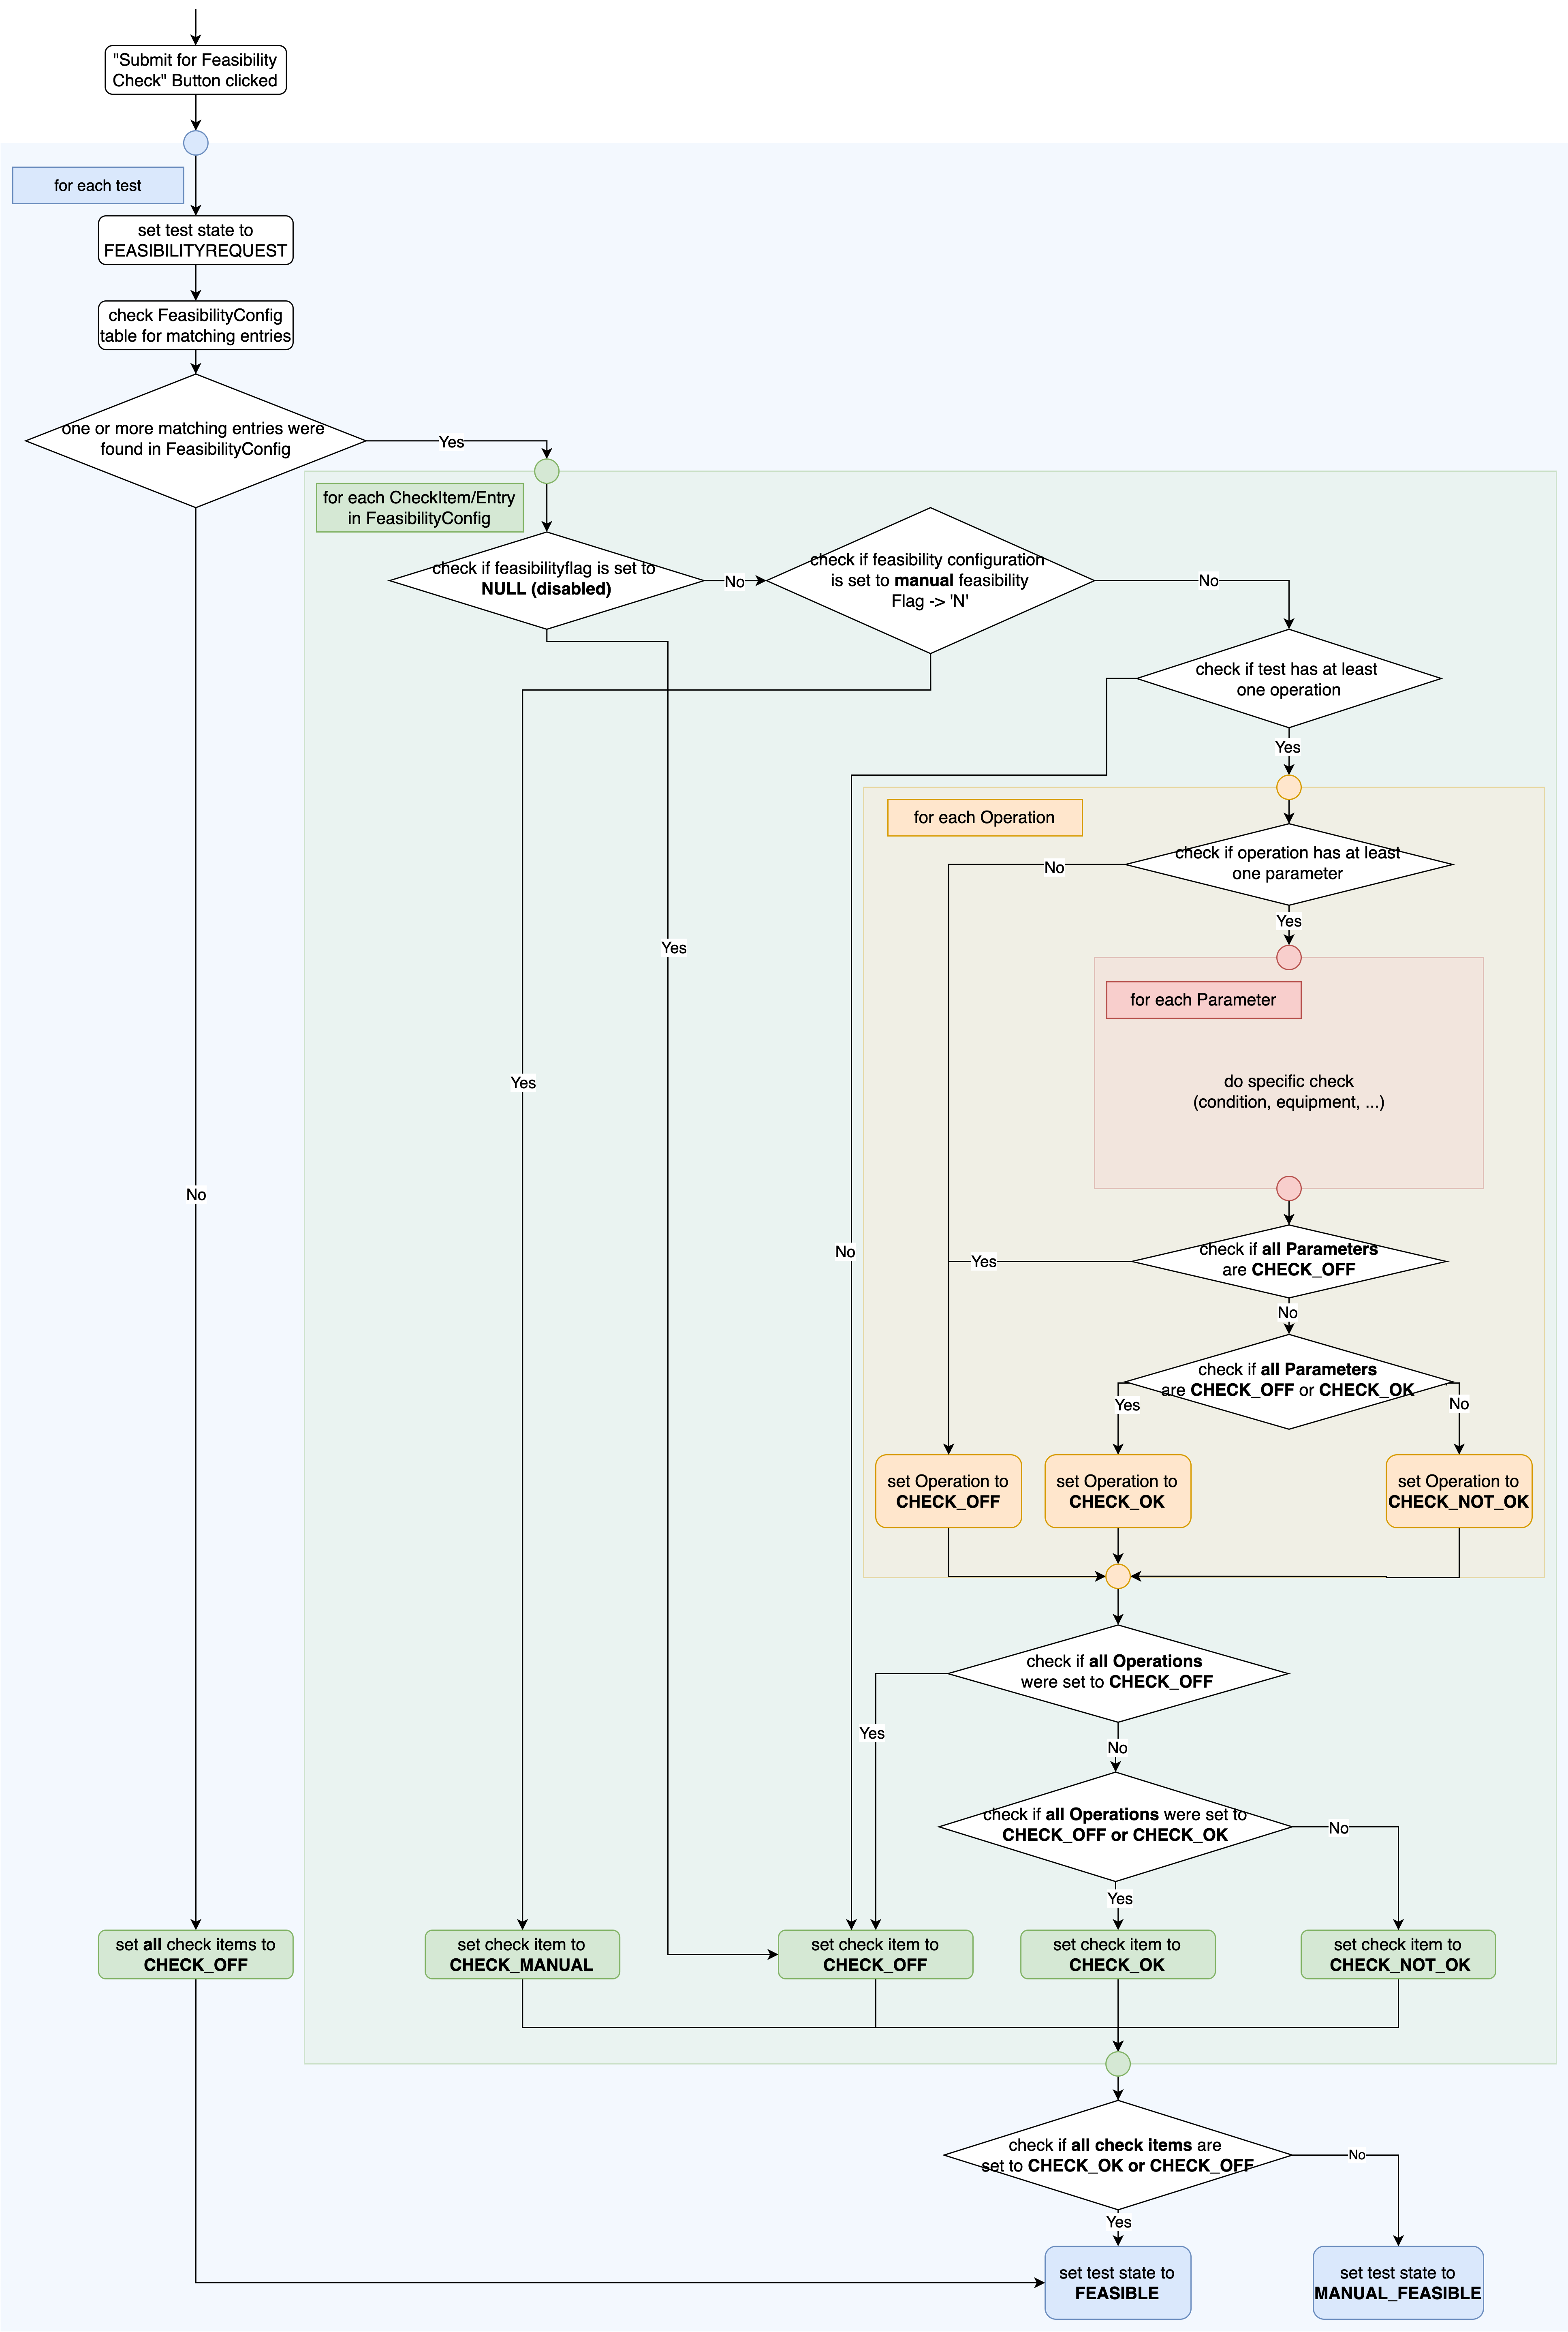
\includegraphics[width=0.85\paperwidth]{bilder/flowchart-feasibilitycheck-without-param-check.png}}
    \caption{Flowchart Feasibility Check - Condition Check }
    \label{fig:feasibility-check-condition-check}
\end{figure}

\section{Frontend-Design}
Überblick über die Angular-Anwendung, Struktur und Benutzeroberfläche.